%!TEX root = ../dokumentation.tex

\chapter{Die iOS App}\label{cha:iOS App}

Dieses Kapitel beschreibt die Struktur und den Aufbau der für die Ansteuerung der Drohne benötigten iOS App. Es wird ein überblick über die verwendete Architektur und Benutzeroberfläche, sowie über die verwendeten Klassen gegeben.

\section{Aufbau}
Die iOS-App ist mit Hilfe des \acs{MVC} Pattern entwickelt. Dadurch gibt sich ein Aufbau aus verschiedenen Controllern und Views. In diesem Projekt gibt es für jede einzelne View einen eigenen Controller. Die Daten, wie die Flugroute sind als Models implementiert. 
\newline
Die Views sind alle in einem Storyboard zu finden. Die Views werden im Kapitel \acs{GUI} genauer beschrieben. 
\newline
Die App stellt die Schnittstelle zum Anwender dar. Darunter sitzt das DJI Mobile SDK, welches Funktionen der Drohne implementiert. Das \acs{SDK} stellt die äußere Schnittstelle zur Drohne dar.
\newline Die Kommunikation zwischen mobilem Endgerät und Drohne wird über die WLAN-Verbindung der Fernbedienung ermöglicht. 

\section{\acf{GUI}}
Die \acs{GUI} besteht aus verschiedenen Views. Die folgende Abbildung zeigt den Aufbau der \acs{GUI} in einem Storyboard. 
\newline
\begin{figure}[H]
	\begin{center}
		{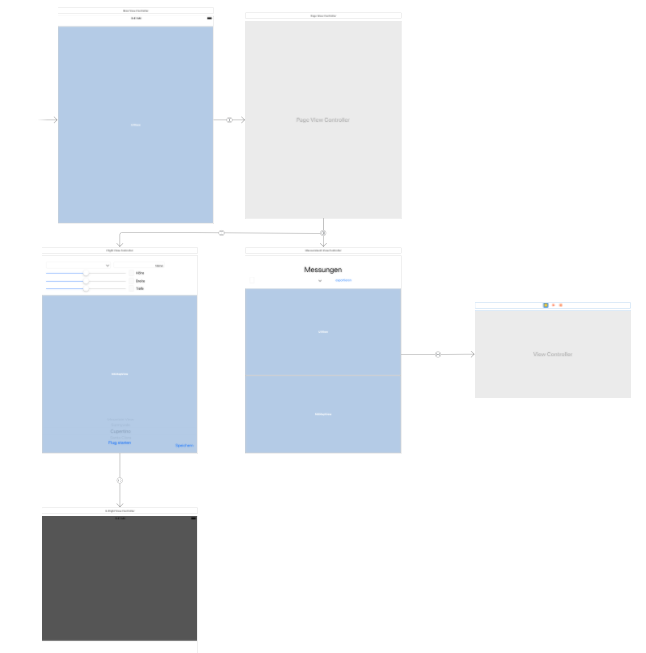
\includegraphics[width=1\textwidth]{images/AufbauGUI.png}}
		\caption{Aufbau \acs{GUI}}
	\end{center}
\end{figure}
\subsection{MainView}
Es gibt eine MainView, welche an der oberen Kante des Displays eine Statusleiste abbildet, die Informationen über den Standort und Zustand der Drohne visualisiert. Neben der Statusleiste beinhaltet die MainView noch eine ContainerView. 
\subsubsection{Statusleiste}
Die Statusleiste bildet genauer folgende Informationen ab. 
\begin{itemize}
	\item Batteriestatus der Drohne
	\item Stärke des WiFi-Signals
	\item Qualität des GPS-Signals
	\item Die aktuelle Flughöhe der Drohne 
	\item Flugstatus
\end{itemize}
Realisiert ist die Statusleiste über Elemente der DJI UXLibrary. Die einzelnen View-Elemente erben von den UXLibrary-Klassen. Die UXLibrary Klassen sind an dem Präfix \textit{\textit{DUL}} zu erkennen. So sind die Obengenannten Widgets durch die UXLibrary Klassen,
\begin{itemize}
	\item DULBatteryWidget
	\item DULWifiSignalWidget
	\item DULGPSSignalWidget
	\item DULAltitudeWidget
	\item DULPreFlightStatusWidget
\end{itemize}
wie folgt realisiert:
\newline
\begin{lstlisting}[caption={Statusleiste}]
@IBOutlet var batteryWidget: DULBatteryWidget!
@IBOutlet var wifiWidget: DULWifiSignalWidget!
@IBOutlet var GPSWidget: DULGPSSignalWidget!
@IBOutlet var altitudeWidget: DULAltitudeWidget!
@IBOutlet var flightStatusWidget: DULPreFlightStatusWidget!
\end{lstlisting}
Die folgende Abbildung zeigt die Darstellung der Statusleiste in der App.
\newline
\begin{figure}[H]
	\begin{center}
		{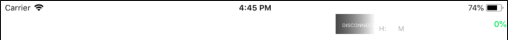
\includegraphics[width=0.5\textwidth]{images/Statusbar.png}}
		\caption{Statusbar}
	\end{center}
\end{figure}
\subsubsection{ContainerView}
Die ContainerView nimmt, außer der Statusleiste am oberen Rand, den restlichen Platz des Displays ein. In die ContainerView werden die anderen Views geladen. Somit bekommt der Anwender in jeder Ansicht, über die Statusleiste, eine Übersicht über den Zustand der Drohne.  
\subsection{PageView}
Um eine Trennung der Ansichten auf die Messungen und auf den Flugbetrieb zu bekommen, wird eine PageView implementiert. Diese PageView beinhaltet eine View für die Messungen und eine weitere View für den Flugbetrieb. 
\newline
Um zwischen der \textit{FlightView} und der \textit{MessearumentView} zu wechseln ist eine einfache Wischgeste notwendig. Man kann die Views unendlich wechseln. Damit ist gemeint, dass man nicht nur einmal nach rechts wischen kann und dann wieder nach links wischen muss, um auf die andere View zu kommen. Egal welche Wischgeste, nach links oder nach rechts, man ausführt, man wechselt die View.
\subsubsection{FlightView}
Die \textit{FlightView} beinhaltet eine Kartenansicht, sowie zwei Slidebars, um die Höhe und Tiefe der abzufliegenden Route auszuwählen. Es soll noch zusätzlich eine Combobox implementiert werden, welche es ermöglicht bereits abgespeicherte Routen auszuwählen. Um eine neue Route mit Namen hinzuzufügen ist ein Textfeld neben der Combobox zu finden. Im unteren Abschnitt befinden sich noch die Buttons \textit{Flug starten} und \textit{Speichern}. 
\newline
Der Button \textit{Speichern} soll bewirken, dass die Flugroute welche man erstellt hat abgespeichert wird. Der Button \textit{Flug starten} soll einen automatischen Drohnenflug starten. Es wird in ein Livefeed der Kamera der Drohne gewechselt. 
\newline
\begin{figure}[H]
	\begin{center}
		{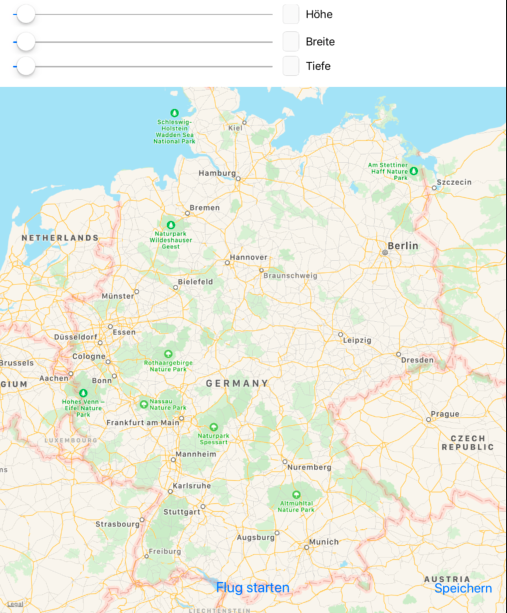
\includegraphics[width=0.5\textwidth]{images/FlightView.png}}
		\caption{FlightView}
	\end{center}
\end{figure}
\subsubsection{MeassurementView}
Die \textit{MessearumentView} besteht aus einer Combobox über die man eine Messung auswählen können sollte. Daneben befindet sich ein Button exportieren, welcher dazu gedacht ist eine Messung als csv-File zu exportieren.
\newline
darunter existiert eine ContainerView welche Platz für eine Tabelle bietet, um die Messwerte als Tabelle anzuzeigen. Darunter existiert wiederum eine Kartenansicht um die Messung in einer Heatmap darzustellen. 
\newline
\begin{figure}[H]
	\begin{center}
		{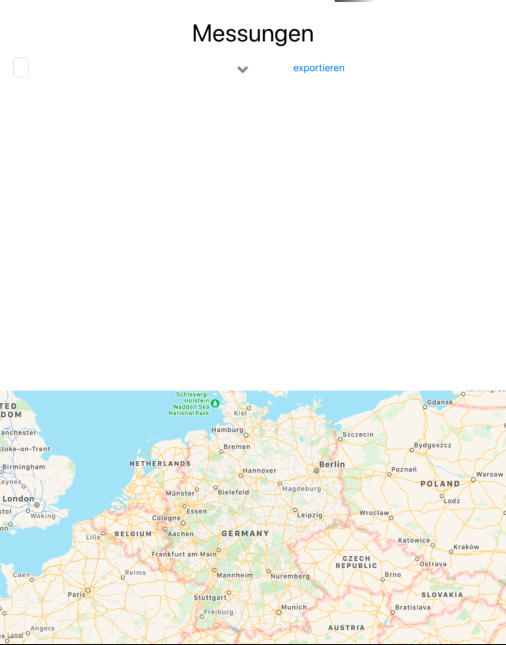
\includegraphics[width=0.5\textwidth]{images/MessearumentView.png}}
		\caption{MessearumentView}
	\end{center}
\end{figure}

\section{Das autonome Fliegen}
Der autonome Flug der Drohne ist über eine sogenannte Waypoint Mission realisiert. Diese beschreibt die Funktion des DJI Mobile SDK, dass die Drohne nacheinander vorgegebene Punkte anfliegt. Diese Mission muss auf die Drohne hochgeladen werden.
\newline
\subsection{Hochladen der Waypoint Mission}
Um eine Waypoint Mission zu starten, muss diese zuerst auf die Drohne hochgeladen werden. Dies geschieht über die \textit{DJIMissionControl}. Die \textit{DJIMissionControl} handhabt das ausführen von verschiedenen Missionen. Es gibt die Möglichkeit zweckbestimmte Mission Operators oder eine Serie von Missionen in einer Zeitachse auszuführen. 
\newline
Die \textit{DJIMissionControl} hat dafür die sogenannten Mission Operators. In dieser Arbeit ist nur der \textit{DJIWaypointMissionOperator} wichtig. Dieser Mission Operator kann über Listener den aktuellen Stand der Mission abfragen. Wie in diesem Projekt das hochladen der Waypoint Mission auf die Drohne implementiert ist, zeigt folgendes Quellcode Beispiel.
\newline
\begin{lstlisting}[caption={Upload und ausführen der Waypoint Mission auf der Drohne}]
func addWaypointMissionToTimeline(waypointMission: DJIMutableWaypointMission) -> Bool {

	var success = false

	let toScheduleWaypointMission = DJIWaypointMission(mission: waypointMission)

	let missionError = toScheduleWaypointMission.checkParameters()

	if missionError == nil {
		NSLog("Mission valide")
	}
	else{
		NSLog("Mission nicht valide: " + (missionError?.localizedDescription)!)
	}

	let errorAddingOperator = DJISDKManager.missionControl()?.waypointMissionOperator().load(toScheduleWaypointMission)
	if errorAddingOperator == nil {
		NSLog("Loaded Mission")
		success = true
	}
	else {
		NSLog("Error loading WPM: " + (errorAddingOperator?.localizedDescription)!)
	}

	if DJISDKManager.missionControl()?.waypointMissionOperator().currentState == DJIWaypointMissionState.readyToUpload
		&& missionOperator.loadedMission?.checkParameters() == nil{
		DJISDKManager.missionControl()?.waypointMissionOperator().uploadMission(completion: { (errorUpload) in
			if errorUpload != nil {
				NSLog("Error Uploading Mission to Aircraft" + (errorUpload?.localizedDescription)!)
			}
			else {
				NSLog("Uploaded Mission to Aircraft")
				//self.addMissionOperatorUpdateListener()
			}
		})
	}
	return success
}

func addMissionOperatorUploadListener() {
	missionOperator.addListener(toUploadEvent: self, with: DispatchQueue.main, andBlock: { (error) in
		if error.error != nil {
			NSLog("Fehler uploading: " + error.description)
		}
		else {
			if self.missionOperator.currentState == .readyToExecute {
				NSLog("Upload Done")
				self.missionOperator.startMission(completion: { (errorExecuting) in
					if errorExecuting != nil {
						NSLog("Fehler bei Ausfuehrung: " + String(describing: errorExecuting))
				}
				else {
					NSLog("Kein Fehler bei Ausführung")
				}

				self.missionOperator.removeAllListeners()
				})
			}
		}
	})
}
\end{lstlisting}
Wurde die Mission erfolgreich hochgeladen, kann diese über den Befehl \textit{missionOperator.startMission()} ausgeführt werden. Im obigen Quellcode Beispiel wurde über den \textit{DJIWaypointMissionOperator}, ein Listener hinzugefügt, welcher überprüft ob die Mission erfolgreich hochgeladen wurde. Ist dies der Fall wird die Mission ausgeführt. 
\newline 
Bevor der Listener hinzugefügt wird, wird die Mission der Zeitachse der \textit{DJIMissionControl} hinzugefügt. War dies erfolgreich wird der Listener hinzugefügt.

\subsection{Erstellen der Waypoint Mission}
Der autonome Flug der Drohne ist in einer \textit{DJIWaypointMission} implementiert. Diese fliegt die in Ihr enthaltene Waypoints an. 
\newline
Bei betätigen des Buttons \textit{Flug starten}, wird eine \textit{DJIWaypointMission} angelegt. Diese beinhaltet noch keine konkreten Waypoints. In dieser Mission werden die Rahmenbedingungen für den gesamten Flug gesetzt. Die Mission ist vom Typ \textit{DJIMutableWaypointMission}, was bedeutet sie kann verändert werden.
\newline
Als für den gesamten Flug geltende Einstellungen werden folgende Parameter der Waypoint Mission gesetzt. Die Waypoint Mission wird mittels der Funktion \textit{createMission()} erstellt, welche im Folgenden zu sehen ist.
\newline
\begin{lstlisting}[caption=Erstellen einer Waypoint Mission]
private func createMission() -> DJIMutableWaypointMission? {
	let mission = DJIMutableWaypointMission()

	mission.autoFlightSpeed = Float(activeFlightRoute.velocity)
	mission.finishedAction = .goHome
	mission.headingMode = .auto
	mission.flightPathMode = .normal
	mission.exitMissionOnRCSignalLost = true
	mission.gotoFirstWaypointMode = .safely
	mission.repeatTimes = 1

	return mission
}
\end{lstlisting}
Die Mission soll genau einmal ausgeführt werden und die Waypoints sollen direkt ohne Umweg angeflogen werden. Die Geschwindigkeit mit der sich die Drohne bewegt wird durch die Messhäufigkeit berechnet. Diese beträgt eine Messung pro Sekunde. Somit kann gewährleistet werden, dass ein regelmäßiges Messgitter entsteht und alle Messungen gleich weit von einander Entfernt durchgeführt wurden. 
\newline
Die Geschwindigkeit berechnet sich aus dem kürzesten Abstand zweier Waypoints. 
\newline
Zum Ende der Mission, soll die Drohne zurück zum Ausgangspunkt fliegen.
\newline
Ist die Waypoint Mission angelegt, werden der Mission die einzelnen Waypoints hinzugefügt. 

\subsection{Berechnen der Waypoints}
Die Waypoints werden automatisch von der aktuellen Position der Drohne aus berechnet. Die maximale Anzahl der Waypoints ist auf 99 begrenzt. 
\newline
Im Allgemeinen wird von einem Rechteck ausgegangen, welches sich vom Standort der Drohne nach Norden und Westen ausbreitet. Die maximale Fläche, welche abgeflogen werden kann ist auf 30m x 30m begrenzt und lässt sich über die Entsprechenden Slider in der \acs{GUI} auswählen. Der Wert width entspricht der Richtung nach Norden, der Wert depth der Richtung nach Westen.
\newline
Aufgrund von Zeitproblemen bei der Implementierung werden immer 6 Luftschichten im Bereich von 1,2 Metern bis 30 Metern abgeflogen. 30 Meter entspricht der maximal erlaubten Flughöhe für Drohnen bis 5 kg in Deutschland.
\newline
Durch das abfliegen der verschiedenen Luftschichten bleiben für jede Luftschicht 16 Waypoints übrig. Das heißt man kann pro Luftschicht 16 Waypoints zum anfliegen verwenden. Dadurch ergibt sich eine mindest Messhäufigkeit. Um ein gelichmäßiges Messgitter zu gewährleisten werden die Waypoints, wie folgt angeflogen.
\newline
\begin{figure}[H]
	\begin{center}
		{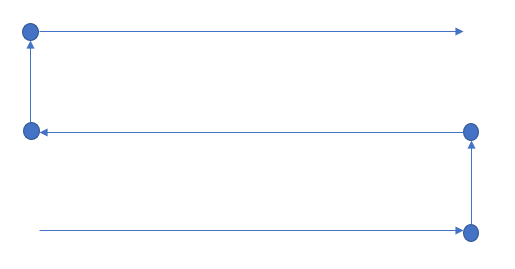
\includegraphics[width=0.5\textwidth]{images/WaypointAufteilung.png}}
		\caption{Anfliegen der Waypoints}
	\end{center}
\end{figure}
Um die begrenzte Anzahl der Waypoints optimal zu nutzen wird zuerst überprüft, welche Strecke der zu messenden Fläche größer ist. Aus der kürzeren Strecke, geteilt durch acht, ergibt sich die Geschwindigkeit mit der sich die Drohne fortbewegt ($v = \frac{s}{t}$ mit s = kurze Distanz; t = eine Messung pro Sekunde). Die Geschwindigkeit legt auch den Mindestabstand der Messungen fest. 
\newline
Die verschiedenen Waypoints werden vom Startpunkt ausgehend, welcher dem HomePoint der Drohne entspricht, berechnet. Die Waypoints werden über \textit{CLLocationCoordinates2D} initialisiert. Deshalb muss die Entfernung von einer Entfernung in der Einheit Meter in eine Entfernung in Längengrad und Breitengrad umgerechnet werden. 
\newline
Hierfür wird die Erde als Kugel angenähert. Dies ist im Fall der Anwendung der App legitim, da die tatsächliche Form der Erde bei Entfernungen von 30 Metern keine Auswirkungen hat. Für die Umrechnung einer Entfernung in Metern in Breitengrad, wird die Entfernung mit dem Faktor 1/111120.0 multipliziert. Für die Umrechnung einer Entfernung in Meter in Längengrad wird die Entfernung mit dem Faktor 1/25700000.0 multipliziert. Die entsprechenden Funktionen sehen wie folgt aus.
\newline
\begin{lstlisting}[caption={Umrechnung Meter in Längengrad und Breitengrad}]
	private func meter2degree_latitude (dist_meter: Double) -> Double {
		var dist_lat: Double
		let lat_const: Double = 111120.0 //Näherung
		dist_lat = dist_meter * (1/lat_const)
	
		return dist_lat
	}
	
	private func meter2degree_longitude (dist_meter: Double) -> Double {
		var dist_long: Double
		let long_const: Double = 25700000.0 //Näherung für Deutschland www.iaktueller.de
		dist_long = dist_meter * (1/long_const)
	
		return dist_long
	}
\end{lstlisting}
Über die erhaltenen Distanzen werden die einzelnen Positionen der Waypoints berechnet und einem Array hinzugefügt. Nach berechnen von 16 Waypoints wird die Höhe um 4,8 Meter erhöht und die Waypoints werden nach gleichem Vorgehen mit einer neuen Flughöhe dem Array hinzugefügt. Somit erhält man 6 verschiedene Waypoints an einer Position mit verschiedener Höhe. 
\newline
Ein Waypoint wird mit den entsprechenden Koordinaten erstellt. Danach werden dem Waypoint Geschwindigkeit und Flughöhe hinzugefügt. 